\documentclass[12pt]{article}
\usepackage{amsmath,graphicx,color,epsfig,physics}
\usepackage{float}
\usepackage{subfigure}
\usepackage{slashed}
\usepackage{bbold}
\usepackage{color}
\usepackage{multirow}
\usepackage{feynmp}
\textheight=9.5in \voffset=-1.0in \textwidth=6.5in \hoffset=-0.5in
\parskip=0pt
\def\del{{\partial}}


\begin{document}

\begin{center}
{\large\bf HW10 for Advanced Particle Physics} \\

\end{center}

\vskip 0.2 in

Dear students,

  Today, I review Higgs interactions in the SM.  Please let me start
  from the flavor diagonal Higgs couplings in the SM.



  \begin{enumerate}
      \item The SM Higgs boson does not have couplings between quarks and leptons
      of different generations (absence of FCNC).  This is because the same
      Unitary matrices that rotates the current states to the mass
      eigenstates rotates the Higgs-fermion-fermion couplings.
      \item The custodial SU(2) symmetry of the Higgs potential can be extended
      to include the Yukawa coupling if the top and the bottom quark masses
      are the same.
      \item Several consequences of custodial SU(2) symmetry and its breaking
      are explained qualitatively.  Serious understanding of the meaning of
      precision measurements is possible only after you study quantization
      of gauge theories and learn techniques to calculate quantum corrections.
      
  \end{enumerate}

  I noticed that it is useful to study $K^0-{\overline K^0}$ mixing at the quark
  amplitude level (without actual calculation) to explain why the
  extreme smallness of the FCNC has been such a critical data which
  led us to the GIM mechanism, and through the CPV study in the same
  amplitudes to the Kobayashi-Maskawa model.

  I also noticed that it is relatively important to study neutrino
  oscillation phenomenology a little bit, in order to know how the
  MNS mixing matrix elements and the mass-squared differences are
  measured.  This is possible without using QFT, since neutrino
  oscillation can be described completely by using quantum mechanics.

  Parametrization of $V_{CKM}$ and $V_{MNS}$:

  I explained in my lectures that 3 by 3 unitary matrix for quark
  charged currents,
  \begin{eqnarray}
    \begin{pmatrix}
      u_L^* & c_L^* & t_L^*
    \end{pmatrix}
    \sigma_-^\mu V_{CKM}
    \begin{pmatrix}
      d_L \\ s_L \\ b_L
    \end{pmatrix}
  \end{eqnarray}
   has 4 real components, since $18-9$ (unitarity) $-5$ (quark phases except for
  the common phase for all $6$ quarks) $= 4$.  This 4 real components are
  parametrized by 3 mixing angles and 1 phase (Kobayashi-Maskawa, 1973).
  \begin{eqnarray}
    V = O_{23} P O_{13} P^* O_{12}
  \end{eqnarray}
  Please note that the 3 orthogonal matrices are not cyclic in their
  parametrization, which is adopted by PDG.  They are defined as:
\begin{eqnarray}
  (O_{23})_{23}&=&\sin\theta_{23} \\
  (O_{13})_{13}&=&\sin\theta_{13} \\
  (O_{12})_{12}&=&\sin\theta_{12} 
\end{eqnarray}
  $P$ is a diagonal phase matrix,
\begin{eqnarray}
  P = {\rm diag}\{ 1, 1, e^{i\delta} \}
\end{eqnarray}

{\bf hw10-1}: Please obtain $V$ in terms of the 3 angles and $\delta$.
  Please compare it with the matrix given in RPP, in
  the review section 12, CKM quark-mixing matrix, {\bf Eq.(12.3)}.

  Because no physical observable can change by changing the
  phases of $u_L$, $c_L$, $s_L$, $b_L$, in the expression
\begin{eqnarray}
  \begin{pmatrix}
    u_L^* & c_L^* & t_L^*
  \end{pmatrix}
  \sigma_-^\mu
  \begin{pmatrix}
    V_{ud} & V_{us} & V_{ub} \\
    V_{cd} & V_{cs} & V_{cb} \\
    V_{td} & V_{ts} & V_{tb}
  \end{pmatrix}
  \begin{pmatrix}
    d_L & s_L & b_L 
  \end{pmatrix}
\end{eqnarray}
  we can choose
  \begin{eqnarray}
    V_{ud}, V_{us}, V_{cb}, V_{tb} > 0
  \end{eqnarray}
  without loss of generality. By comparing the 4 elements with the
  standard parametrization of {\bf hw10-1},

{\bf hw10-2}: please show that the ``defined region'' of the 3 angles can be
\begin{eqnarray}
  0 \le \theta_{23}, \theta_{13}, \theta_{12} < \pi/2
\end{eqnarray}
  
  Let us show why Weinberg could not apply his model to quarks (he called his MSM as a model for leptons).  By the time of his studies in 1967, it was found by Cabibbo (1964) that all the known weak charged current interactions can be obtained from
  \begin{eqnarray}
    {\cal L}_{CC}
  =
  \frac{-g}{\sqrt{2}} W^-_\mu (e_L^\dagger)  \sigma_-^\mu \nu_e +
  \frac{-g}{\sqrt{2}} W^-_\mu (\mu_L^\dagger) \sigma_-^\mu \nu_\mu +
  \frac{-g}{\sqrt{2}} W^+_\mu (u_L^\dagger)  \sigma_-^\mu d_L'
  + h.c.
  \end{eqnarray}  
   where by introducing the combination
\begin{eqnarray}
  d_L' = \cos\theta_C d_L + \sin\theta_C s_L
\end{eqnarray}
  Cabibbo showed that all three terms have exactly the same strengths
  (more precisely, he showed that the product of $e_L-\nu_e$ current and
  $\mu_L-\nu_\mu$ current has the same strength as the product of $e_L-\nu_e$ current and the $u_L-d_L'$ current). This universality of the charged currents between quarks and leptons motivated everybody to look for the gauge
  theory of weak interactions.  Weinberg was the first physicist who
  succeeded on this.

  But as we showed in {\bf hw09-5}, this model with 3 quarks gives the Z boson
  coupling as
\begin{eqnarray}
  &&-g_Z Z_\mu [(\frac{1}{2}-\frac{2}{3}x_W) u_L^\dagger  \sigma_-^\mu u_L
  + (-\frac{1}{2}-\frac{-1}{3}x_W) {d'_L}^\dagger \sigma_-^\mu d_L' \nonumber\\
  &&+ (    -\frac{2}{3}x_W) u_R^\dagger  \sigma_+^\mu u_R
  + (    -\frac{-1}{3}x_W) d_R^\dagger  \sigma_+^\mu d_R ]
\end{eqnarray}

The above interactions contain the $Z-d_L-s_L$ (FCNC) coupling:
\begin{eqnarray}
  -g_Z Z_\mu (-1/2+(1/3)x_W) \cos\theta_C \sin\theta_C
[ d_L^\dagger \sigma_-^\mu s_L + s_L^\dagger \sigma_-^\mu d_L ]
\end{eqnarray}
This term contributes to the $K_0-{\overline K_0}$ transition,
\begin{eqnarray}
  K_0(d \bar s) \to {\overline K_0}( \bar d s)
\end{eqnarray}
  by a Z-boson exchange, with the amplitude proportional to
\begin{eqnarray}
  \frac{g_Z^2}{m_Z^2} (-\frac{1}{2}+(\frac{1}{3}x_W)^2 (\cos\theta_C \sin\theta_C)^2
  =
  G_F \times 8 (-\frac{1}{2}+(\frac{1}{3}x_W)^2 (\cos\theta_C \sin\theta_C)^2
\end{eqnarray}
  This contributes to the $K_L-K_S$ mass difference at the level of 
  \begin{eqnarray}
    m_K^2 G_F = (0.5 GeV)^2 (10^{-5} GeV^{-2}) = 10^{-7},
  \end{eqnarray} 
  in comparison to the measurement
  $(m(K_L)-m(K_S))^2/m_K^2 = 10^{-20}$.
  This huge discrepancy between the prediction of Weinberg's model with
  Cabibbo universality, made him abandoned the idea of proposing his
  model for all the particles including hadrons.

  In the 4-quark model of GIM (1971), as we showed above, the cancellation
  of $2 \times 2$ Unitary matrices makde all the Z-q-q couplings diagonal.  There is no $Z-d-s$ couplings.

  Immediately after t'Hooft proved the renormalizability of the
  electroweak theory in 1971, Lee and Gaillard calculated the $K^0-{\overline K^0}$ mixing in the 4-quark model at one-loop level. It is something like Fig.\ref{fig.101}:
  \begin{figure}[htb]
    \centering
    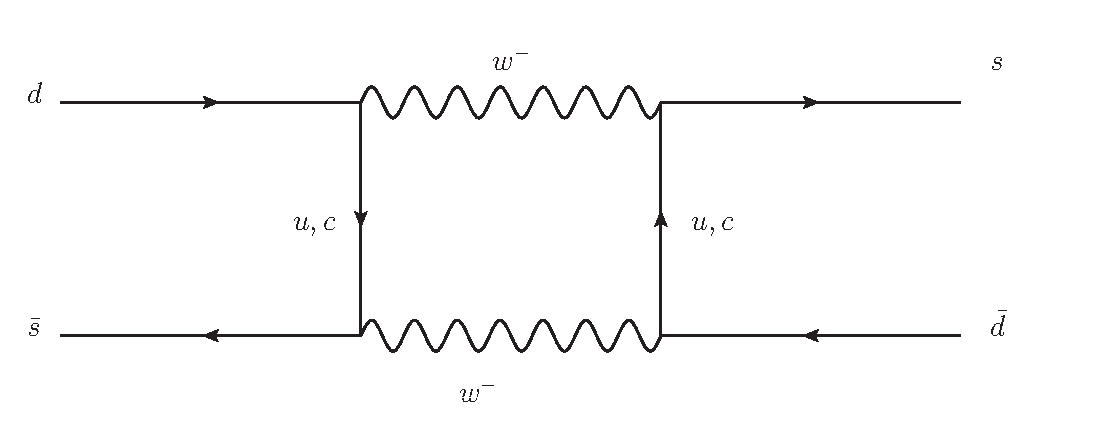
\includegraphics[scale=0.6]{hw10.eps}
    \caption{ }\label{fig.101}
  \end{figure}
  The amplitude is very naively expressed as
\begin{eqnarray}
  (g/\sqrt{2})^4/(m_W)^4 \times [ V_{ud} V_{us}^* f(m_u) + V_{cd} V_{cs}^* f(m_c) ]^2
\end{eqnarray}
  where $f(m_u)$ and $f(m_c)$ corresponds to the contribution of the up quark
  and charm quark, respectively.  If $m_c=m_u$, $f(m_u) = f(m_c)$, and the
  contribution vanishes since
\begin{eqnarray}
  V_{ud} V_{us}^* + V_{cd} V_{cs}^* = (V^\dagger V)_{sd} = 0
\end{eqnarray}
   from the Unitarity of the $2 \times 2$ mixing matrix.  Therefore it reads
\begin{eqnarray}
  (g/\sqrt{2})^4/(m_W)^4 (V_{ud} V_{us}^*)^2 \times [ f(m_u) - f(m_c) ]^2
\end{eqnarray}
  Although I don't remember details, the last factor is proportional to
\begin{eqnarray}
  ((m_u^2 - m_c^2)/m_W^2)^2 = m_c^4/m_W^4
\end{eqnarray}
  or
\begin{eqnarray}
  ((m_u - m_c)/m_W)^2 = m_c^2/m_W^2
\end{eqnarray}
  and Lee and Gaillard could predict the charm quark mass to be around
  $2$GeV, by comparing their calculation and the $K_L-K_S$ mass difference.
  Please find the paper by B.W.Lee and M.Gaillard (1972), and compare
  my expressions above and theirs. I may have missed some factors.\\


  In the minimum SM, the absence of FCNC Higgs coupling is guaranteed
  since all the quark and lepton masses are generated by only one v.e.v.,
\begin{eqnarray}
  {\rm masses} = {\rm coupling} \times v
\end{eqnarray}
  and the Higgs boson couplings appear by the replacement $v \to v+h$

  Since the mass terms among the mass-eigenstates are diagonal by
  definition, all the Higgs interactions are also diagonal, whose
  strength is proportional to
  $mass/v$
  When we consider models beyond the SM, it is very important to keep
  the flavor diagonality of all the interactions, including extended
  gauge interactions and the extended Higgs interactions.

{\bf hw10-3}: In {\bf hw09}, I asked you to express the Higgs Lagrangian
\begin{eqnarray}
  {\cal L}_{Higgs} = (D_\mu \phi)^\dagger (D^\mu \phi) - V(\phi)
\end{eqnarray}
   by inserting the v.e.v.,
\begin{eqnarray}
  <\phi> =
  \begin{pmatrix}
    0 \\ v/\sqrt2
  \end{pmatrix}
\end{eqnarray}
  Please obtain ${\cal L}_{Higgs}$ again, now for the Unitary gauge $\phi$,
\begin{eqnarray}
  \phi = 
  \begin{pmatrix}
    0 \\ (v+H)/\sqrt2
  \end{pmatrix}
\end{eqnarray}

{\bf hw10-4}:
  When we parametrize the above ${\cal L}_{Higgs}$ as
\begin{eqnarray}
  {\cal L}_{Higgs} &=& \frac{1}{2} \del_\mu H \del^\mu H+
              m_W^2 W^+_\mu {W^-}^\mu
              + \frac{m_Z^2}{2} Z_\mu Z^\mu
              + g_{HWW} H W^+_\mu {W^-}^\mu
              \nonumber \\ &&+ \frac{g_{HZZ}}{2} H Z_\mu Z^\mu
              + \frac{g_{HHWW}}{2} HH W^+_\mu {W^-}^\mu
              + \frac{g_{HHZZ}}{4} HH Z_\mu Z^\mu
              \nonumber \\ &&- \frac{m_H^2}{2} H^2
              - \frac{g_{HHH}}{3!} H^3
              - \frac{g_{HHHH}}{4!} H^4,
\end{eqnarray}
  please express $m_W$, $m_Z$, $m_H$, $g_{HWW}$, $g_{ZWW}$, $g_{HHWW}$, $g_{HHZZ}$, $g_{HHH}$ and $g_{HHHH}$ in terms of $v$, $g$, $g_Z$, $\lambda$.

  When we diagonalize the Yukawa matrices to obtain the relationship
  between the mass eigenstates and the ``current'' states,
\begin{eqnarray}
  {\cal L}_{Yukawa} &=&
  -u_L^\dagger M^u u_R + d_L^\dagger M^d d_R + l_L^\dagger M^l l_R + h.c. \\
  &=&
  -(u_L^\dagger, c_L^\dagger, t_L^\dagger) {\rm diag}\{m_u,m_c,m_t\} (u_R,c_R,t_R)^T\nonumber \\
  &&-(d_L^\dagger, s_L^\dagger, b_L^\dagger) {\rm diag}\{m_d,m_s,m_b\} (d_R,s_R,b_R)^T \nonumber \\ &&- (e_L^\dagger, \mu_L^\dagger, \tau_L^\dagger) {\rm diag}\{m_e,m_\mu,m_\tau\} (e_R,\mu_R,\tau_R)^T
  +
  h.c. \label{eq.10Lyukdiag}
\end{eqnarray}
  
  Please observe that the Higgs-quark-quark couplings are also
  diagonarlized at the same time, because they are obtained
  simply by the replacement
\begin{eqnarray}
  v \to v + H = v(1+H/v)
\end{eqnarray}

{\bf hw10-5}: Please obtain all the H-fermion-fermion couplings by making the replacement
\begin{eqnarray}
  m_f \to m_f (1+H/v)
\end{eqnarray}
   in the above Lagrangian (Eq.\ref{eq.10Lyukdiag}). When we write the $H-f-f$ couplings as
\begin{eqnarray}
  {\cal L}_{Hff} = - \sum_f g_{Hff} H (f_L^\dagger f_R + f_R^\dagger f_L)
\end{eqnarray}
  give $g_{Hff}$ in terms of $m_f$ and $v$, for all $f$={$u$, $d$, $s$, $c$, $b$, $t$, $e$, $\mu$, $\tau$}.

{\bf hw10-6}: Please show also, that the expression for Majorana neutrinos,
\begin{eqnarray}
  {\cal L}_{H\nu\nu} = - \sum_{k=1,2,3} \frac{g_{Hkk}}{2} H (\nu_k \cdot \nu_k)
\end{eqnarray}
  is different, when expressed in terms of $m_k$ ($k=1,2,3$) and $v$, because
  the Majorana neutrino mass is not proportional to $v$, but to $v^2$.  Can
  we use the difference in the $H\nu\nu$ couplings to test Majorana vs Dirac?


  When we consider violation of the classical level prediction of the
  custodial $SU(2)$ symmetry, we often express it as deviation of the
  Veltman's $\rho$ parameter from unity,
  \begin{eqnarray}
    \rho = \frac{G_{NC}}{G_{CC}}=\frac{ g_Z^2/m_Z^2}{g^2/m_W^2} = \frac{m_W^2}{m_Z^2 \cos^2\theta_W}
  \end{eqnarray}
  Since radiative corrections are proportional to the coupling constants,
  we need to consider only the largest of all the Higgs boson couplings,
  which are the HWW and HZZ couplings as well as the Yukawa couplings
  of the 3'rd generation quarks:
\begin{eqnarray}
  y^t &=& -\sqrt{2} m_t/v \\
  y^b &=& -\sqrt{2} m_b/v
\end{eqnarray}
  If we retain only the above two couplings of the Higgs boson to the
  quarks, the Yukawa Lagrangian is simplified as
\begin{eqnarray}
  {\cal L}_{Yukawa} =  y^t (t_L^\dagger,b_L^\dagger) \phi^c t_R
                + y^b (t_L^\dagger,b_L^\dagger) \phi   b_R
                + h.c. \label{eq.10lyuksp}
\end{eqnarray}
  If we take the limit
\begin{eqnarray}
  y^t = y^b = y \label{eq.10ylimt}
\end{eqnarray}
  then Eq.\ref{eq.10lyuksp} can be expressed as
\begin{eqnarray}
  {\cal L}_{Yukawa} &=& y
  \begin{pmatrix}
    t_L^\dagger & b_L^\dagger
  \end{pmatrix}
  (\phi^c t_R + \phi b_R) + h.c. \\
  &=& y 
  \begin{pmatrix}
    t_L^\dagger & b_L^\dagger
  \end{pmatrix}
  \begin{pmatrix}
    \phi^c & \phi
  \end{pmatrix}
  \begin{pmatrix}
    t_R \\ b_R
  \end{pmatrix}+h.c.\\
  &=& y 
  \begin{pmatrix}
    t_L^\dagger & b_L^\dagger
  \end{pmatrix}
  \Phi
  \begin{pmatrix}
    t_R \\ b_R
  \end{pmatrix} +h.c.\label{eq.10yukalmt}
\end{eqnarray}
  The quartet field $\Phi$ %Eq.\ref{eq.8quarfild}
  we introduced in {\bf hw08} appears. It is clear
  that Eq.\ref{eq.10yukalmt} is invariant under the joint transformation,
\begin{eqnarray}
  &&\Phi \to \Phi' = (U_L) \Phi U_R^\dagger \label{eq.10jotran1}\\
  &&(t_L, b_L)^T \to (t_L', b_L')^T = U_L (t_L, b_L)^T  \label{eq.10jotran2} \\
  &&(t_R, b_R)^T \to  (t_R', b_R')^T = U_R (t_R, b_R)^T  \label{eq.10jotran3}
\end{eqnarray}
 
{\bf hw10-7}: Show the invariance of $L_{Yukawa}$ (Eq.\ref{eq.10lyuksp}) under the transformation Eq.(\ref{eq.10jotran1},\ref{eq.10jotran2},\ref{eq.10jotran3}), when $y_t = y_b$ (Eq.\ref{eq.10ylimt}).
Recalling that Eq.\ref{eq.10jotran1} is the symmetry of the Higgs potential 
%(Eq.\ref{eq.8joitran}) 
in {\bf hw08}, we can tell that in the limit of Eq.\ref{eq.10ylimt}, the Yukawa coupling
satisfies the custodial $SU(2)$ symmetry after the symmetry breaking.
Therefore, in this limit, the $\rho$ parameter should not deviate from
unity by the quantum corrections due to Yukawa interactions. With
explicit calculation, we find
\begin{eqnarray}
  \rho - 1 = const. [{y^t}^2 - {y^b}^2]/(4\pi)^2
               = const. [m_t^2 - m_b^2]/[(2v^2)(4\pi)^2]
\end{eqnarray}
  This quantum correction has been found to agree with the precision
  measurements of the $W$ and $Z$ boson masses and their coupling strengths.
  Indeed, the large top quark mass of
\begin{eqnarray}
  m_t = {\cal O}(100GeV)
\end{eqnarray}
   had been predicted from the above quantum corrections, before the top
  quark was discovered in 1994. This was a great success of the
  renormalizable theory of the elctroweak interactions, the Weinberg-Salam
  model.  The successful observation of the quantum corrections not only
  proved the renormalizable theory of spontaneous gauge symmetry breaking,
  but also the presence of the custodial $SU(2)$ symmetry in the symmetry
  breaking interactions.


  Let us obtain the $\rho$ parameter when a different Higgs multiplets
  exist.  Let us assume that there is an additional (doublet is necessary
  to give masses to quarks and charged leptons, since their left-handed
  components are doublets and their right-handed components are singlets)
  Higgs boson, whose weak iso-spin ($SU(2)_L$ quantum number) is
  $T$ ($T=1/2$ for doublets, 1 for triplets, $3/2$ for quartets,
  ...) and its $T^3=-y$ component obtains a v.e.v.
\begin{eqnarray}
  <\phi_k> = \frac{v_k}{\sqrt{2}} {\rm unit}(T_k,T^3=-y_k)
\end{eqnarray}
  
  Here ${\rm unit}(T_k,T^3=-y_k)$ is a column vector normalized to 1, which has
  $2T_k+1$ components, and satisfies
\begin{eqnarray}
  &&[{T^1}^2 + {T^2}^2 + {T^3}^2]            {\rm unit}(T_k,T^3=-y_k)                      = T_k (T_k + 1) {\rm unit}(T_k,T^3=-y_k) \\
  &&Y   {\rm unit}(T_k,T^3=-y_k) =           y_k {\rm unit}(T_k,T^3=-y_k) \\
   &&T^3 {\rm unit}(T_k,T^3=-y_k) =          -y_k {\rm unit}(T_k,T^3=-y_k)
\end{eqnarray}
  

  The above conditions ensure that $<\phi_k>$ does not break $U(1)_{EM}$:
\begin{eqnarray}
  Q <\phi_k> = (T^3+Y) <\phi_k> = 0
\end{eqnarray}
  Now, let us obtain the W and Z masses from the invariant Lagrangian
  of the Higgs boson $\phi_k$:
\begin{eqnarray}
  (D^\mu \phi_k)^\dagger (D_\mu \phi_k)
\end{eqnarray}
 
  We first find,
\begin{eqnarray}
  D_\mu <\phi_k>
  = \frac{ig_W}{\sqrt2} (T^+ W^+_\mu + T^- W^-_\mu) <\phi_k>
  + ig_Z       T^3 Z_\mu<\phi_k>
\end{eqnarray}
  since $\del_\mu <\phi_k> = 0$, and $Q=0$.  We then find immediately,
\begin{eqnarray}
  (D^\mu <\phi_k>)^\dagger (D_\mu <\phi_k>)
  &=& (g_W/\sqrt2)^2 <\phi_k>^\dagger W^-_\mu {W^+}^\mu
                              ( T^- T^+ + T^+ T^- ) <\phi_k> \nonumber \\
  &&+ (g_Z)^2 <\phi_k>^\dagger Z_\mu Z^\mu (T^3 T^3)  <\phi_k> \\
  &=& (g_W v_k/2)^2 W^-_\mu {W^+}^\mu
    {\rm unit}(T_k,-y_k)^T ( T^- T^+ \nonumber \\ &&+ T^+ T^- ) {\rm unit}(T_k,-y_k) + (g_Z v_k)^2/2 Z_\mu Z^\mu \nonumber \\
    && {\rm unit}(T_k,-y_k)^T (T^3)^2 {\rm unit}(T_k,-y_k)
\end{eqnarray}
  
{\bf hw10-8}:  Show the above result.
  From the definition of ${\rm unit}(T_k,-y_k)$, it is clear that
\begin{eqnarray}
  {\rm unit}(T_k,-y_k)^T (T^3)^2 {\rm unit}(T_k,-y_k)
  = (y_k)^2  {\rm unit}(T_k,-y_k)^T {\rm unit}(T_k,-y_k)
  = (y_k)^2
\end{eqnarray}
  The W mass term is slightly more difficult.  In case of the SM Higgs
  boson, since I chose the vacuum expectation value at $T^3=-Y=-1/2$,
  $<\phi(T=1/2,T^3=-1/2)>$, we found
\begin{eqnarray}
  &&{\rm unit}(1/2,-1/2)^T ( T^- T^+ + T^+ T^- ) {\rm unit}(1/2,-1/2) \nonumber\\
  &=& {\rm unit}(1/2,-1/2)^T ( T^- T^+ ){\rm unit}(1/2,-1/2)  
  = 1
\end{eqnarray}
 

  In general, if $T^3=-y_k$ state is not the minimum or the maximum $T^3$
  states ($T^3=\pm T_k$), both terms survive, and we should compute the
  normalization of the upper and lower states.  This problem can be
  bypassed if we note
\begin{eqnarray}
  T^- T^+ + T^+ T^-
  &=& 2 [(T^1)^2 + (T^2)^2 ] \\
  &=& 2 [(T^2)^2 + (T^2)^2 + (T^3)^2] - 2(T^3)^2
\end{eqnarray}
  whose matrix elements should be
\begin{eqnarray}
  {\rm unit}(T_k,-y_k)^T ( T^- T^+ + T^+ T^- ) {\rm unit}(T_k,-y_k)
  = 2 [ T_k(T_k+1) - (y_k)^2 ]
\end{eqnarray}
 
{\bf hw10-9}: Show the above result, and confirm that it agrees with our
  minimum SM W mass, where $T_k=1/2$ and $|y_k|=1/2$.

  We now find
\begin{eqnarray}
  m_W^2 &=& \sum_k (g_W v_k/2)^2 2 [ T_k(T_k+1) - (y_k)^2 ] \\
  m_Z^2 &=& \sum_k (g_Z v_k/2)^2 (y_k)^2
\end{eqnarray}
  after summing over all the Higgs boson $\phi_k$ contributions.
  By using the SM $v^2$ value,
\begin{eqnarray}
  v^2 = 4 m_W^2/g_W^2 = (246GeV)^2
\end{eqnarray}
  as the normalization, we obtain a following compact expression
\begin{eqnarray}
  1-1/\rho = 2 [T_k(T_k+1)]-3(y_k)^2 (v_k/v)^2
\end{eqnarray}

{\bf hw10-10}: Derive the above equation.  Show that the right hand side is
  zero for $T_k=|y_k|=1/2$.  Therefore, the iso-spin $1/2$ doublet Higgs
  boson automatically satisfies $\rho=1$.  How about the Higgs triplet,
  $\phi(T=1,Y=-1)$ and $\phi(T=1,Y=0)$ ?  Can you make a $\rho=1$ model by
  choosing $v(T=1,Y=-1)$ and $v(T=1,Y=0)$ appropriately ?

That's all of hw10.\\

Best regards,\\

Kaoru


\end{document}
